\thispagestyle{empty}

Bugs kill.  Testing software permits to reveal the presence of bugs,
but only formal verification can guarantee their absence.  Thus, the
trust in critical systems today relies on formal verification, in
particular formal proofs, that guarantee the safety of the people
using transportation systems (autonomous cars, subways, trains,
planes, etc.), health systems (robotic surgery, etc.), energy provided
by nuclear plants, financial applications, e-governance, etc.  We
should never fly in an autonomous plane driven by a piece of software
that has not been formally verified.

This crucial role of formal proof is highlighted by several successes,
like the correctness proofs of the automatic Paris metro line 14
\cite{metro14}, the detect-and-avoid system for unmanned aircraft
system developed by NASA \cite{Munoz16}, the operating system seL4
\cite{Klein09}, or the C compiler CompCert \cite{Leroy06}.  It has
been empirically observed that compilers and operating systems often
have bugs, but proved ones, such as seL4 or CompCert, have none, or
much fewer.  This is why, at the highest Evaluation Assurance Levels
of the Common Criteria security evaluation international standard, in
effect since 1999, certification processes require proofs, and not
only testing.

Because a bug can cause people to die and companies to go bankrupt,
formal methods are crucial in the development of the information
society, and hence it is crucial for Europe to master this technology
and its evolution.

Proofs have also always been the basis of mathematics, and hence of
many mathematised sciences, and several important advances, are based
on formal proofs, such as the proof of the Feit-Thompson theorem
\cite{Gonthier13} and Hales' theorem (Kepler's conjecture)
\cite{Hales17}, show the wide range of applications of formal proofs,
from safety and security of software to mathematics.

These formal proofs are developed using research infrastrucures called
``proof systems''.  These proof systems allow computer scientists,
mathematicians, engineers, and logicians to build and study formal
proofs, just like particle accelerators allow physicists to build and
study particles.  Some twenty major proof systems exist in the world
(Figure \ref{systems}).

\begin{center}
  
$\bigstar$ $\bigstar$ $\bigstar$

\end{center}

A lot of formal proofs developed for one critical system could be used
in another.  Unfortunately, the development of formal methods is
slowed down by the large number of proof systems (and sometimes the
large number of versions, over time, of one single system) and the
lack of a common theory used by these systems.  For instance, the
Paris metro line 14 has been proved correct in Atelier B, while the
Nasa detect-and-avoid system for unmanned aircraft system has been
proved correct in PVS, the seL4 operating system has been proved
correct in Isabelle/HOL, and the compiler CompCert has been proved
correct in Coq.  Some projects, such as the proof of Hales' theorem,
have been started in different systems and required significant
integration effort for obtaining the overall result.

Thus, the development of formal methods is slowed down by the lack of
integration of these research infrastructures.  Because of this lack
of integration, each small community is centered around one theory and
one system. Each library is specific to one proof system, or often
even to a specific version of this system. In general, a library
developed in one system cannot be used in another, and when the system
is no longer maintained, the library may disappear.  Thus,
interoperability (the possibility for one user to use a proof
developed in another system), sustainability (the possibility to use a
proof decades after it has been developed), and cross-verification
(the possibility to verify a proof in a system different from that in
which it has been constructed, thus giving a higher assurance of its
correctness) are restricted.

The fragmentation of these infrastucutures hinders productivity
because foundational work (for instance, developing a calculus library
with theorems about the sinus and cosinus functions, derivatives,
etc.) has to be repeated instead of being reused.  It also limits the
spreading of formal proofs in non-specialist communities. For
instance, teaching formal proving to undergraduate students in a logic
course is difficult, as it requires the choice of a specific language,
a specific theory and a specific system that orients the course
towards this language, theory, and system, instead of orienting it to
fundamental principles that are useful everywhere. The same is true
for the use of formal proofs in industry or by working mathematicians.

On more philosophical grounds, while we had in the past an (informal)
proof of Pythagoras' theorem or Fermat's little theorem, the same
proof now has different formalizations in PVS, Isabelle/HOL, Coq, etc.
Thus, the universality of logical truth itself is jeopardized.  As we
shall see, it is not the first time in history that this universality
of logical truth is jeopardized: it already has been, for instance, in the
19$^{\mbox{\footnotesize th}}$ century, with the non-Euclidean
geometries. This crisis of the non-Euclidean geometries has been
solved at the beginning of the 20$^{\mbox{\footnotesize th}}$ with the
invention of a logical framework: predicate logic
\cite{HilbertAckermann}, in which the various geometries could be
defined.

\begin{figure}
\begin{framed}
\begin{center}
\begin{tabular}{l@{\hspace{3cm}}l}
Abella                & Acl 2\\
\underline{Agda}      & \underline{HOL Light}\\
\underline{Atelier B} & IMPS\\
\underline{Coq}       & Lean\\
\underline{FoCaliZe}  & \underline{LFSC}\\
\underline{HOL4}      & Nuprl\\
\underline{Isabelle}  & \underline{PVS}\\
\underline{K Prover}  & \underline{TSTP}\\
\underline{Matita}\\
\underline{Minlog}\\
\underline{Mizar}\\
ProB\\
\underline{ProvenTools}\\
\underline{Rodin}\\
\underline{TLA+}\\
\underline{Why3}\\
\end{tabular}
\end{center}

\caption{Some major proof systems. The European ones are in the first column.
  Those addressed in the project are underlined\label{systems}}
\end{framed}
\end{figure}

\begin{center}
  
$\bigstar$ $\bigstar$ $\bigstar$

\end{center}

Making proof systems interoperable would avoid duplication of work,
reduce development time, enable cross-verification, and make formal
proofs accessible to a much larger community.  After three decades
dedicated to the development of these systems, allowing such a
cooperation between systems is the next step in the development of the
formal proof technology.

Each proof system comes with its own libraries, and these libraries
are also part of research infrastructure.  To address the challenge of
improving cooperation between these proof systems, we will integrate
these libraries in an online encyclopedia of formal proofs. Each proof
in this encyclopedia will have versions in each theory where it can be
expressed, so that it can be used in as many systems as possible.

Each proof system implements a different theory. So Logipedia will
encyclopedia contain proofs expressed in different theories.  Such a
theory-independent infrastructure is made possible, because the
theories implemented in these different proof systems can be expressed
in a common logical framework: the $\lambda \Pi$-calculus modulo
theory, implemented in the system Dedukti.  Dedukti is thus the {\em
lingua franca} that permits this theory-independent encyclopedia to 
exist.

Building such an encyclopedia will thus allow interoperability,
sustainability, and cross-verification of all formal proofs in the
encyclopedia.

This encyclopedia will be called Logipedia.

Logipedia is thus a research infrastructure that integrates proof
systems, through the sharing of data in the form of formal proofs.

\begin{center}
  
$\bigstar$ $\bigstar$ $\bigstar$

\end{center}

Such an infrastructure is, in many ways, new in the European Strategy
on Research Infrastructures. We can even say that the idea to
structure a networking activity around the construction and the use of
a large scale infrastructure is relatively new in computer science and
mathematics, even if other projects, such as {\em OpenDreamKit} and
{\em Software Heritage} do exist.

Our goal is therefore also trigger a
small, but significant, evolution on the organization of research in
computer science and mathematics in Europe.

\begin{framed}
  \vspace*{-0.5cm}
  \begin{center}
{\bf \Large History of the project}
\end{center}

Convinced that a cloud of formal proofs could bring to the
applications of formal proof technology the same boost that the cloud
has brought to computing, and also that managing a large encyclopedia
required some interdisciplinary effort,
we developed a proof of concept containing a few hundreds lemmas
expressed in the language of six systems and organized, in January 2019,
a meeting to discuss the future of this project.
This
meeting brought together 38 researchers from Austria, the Czech
Republic, France, Italy, the Netherlands, and Poland, some of them
being from the TYPES community, others not.
\begin{center}
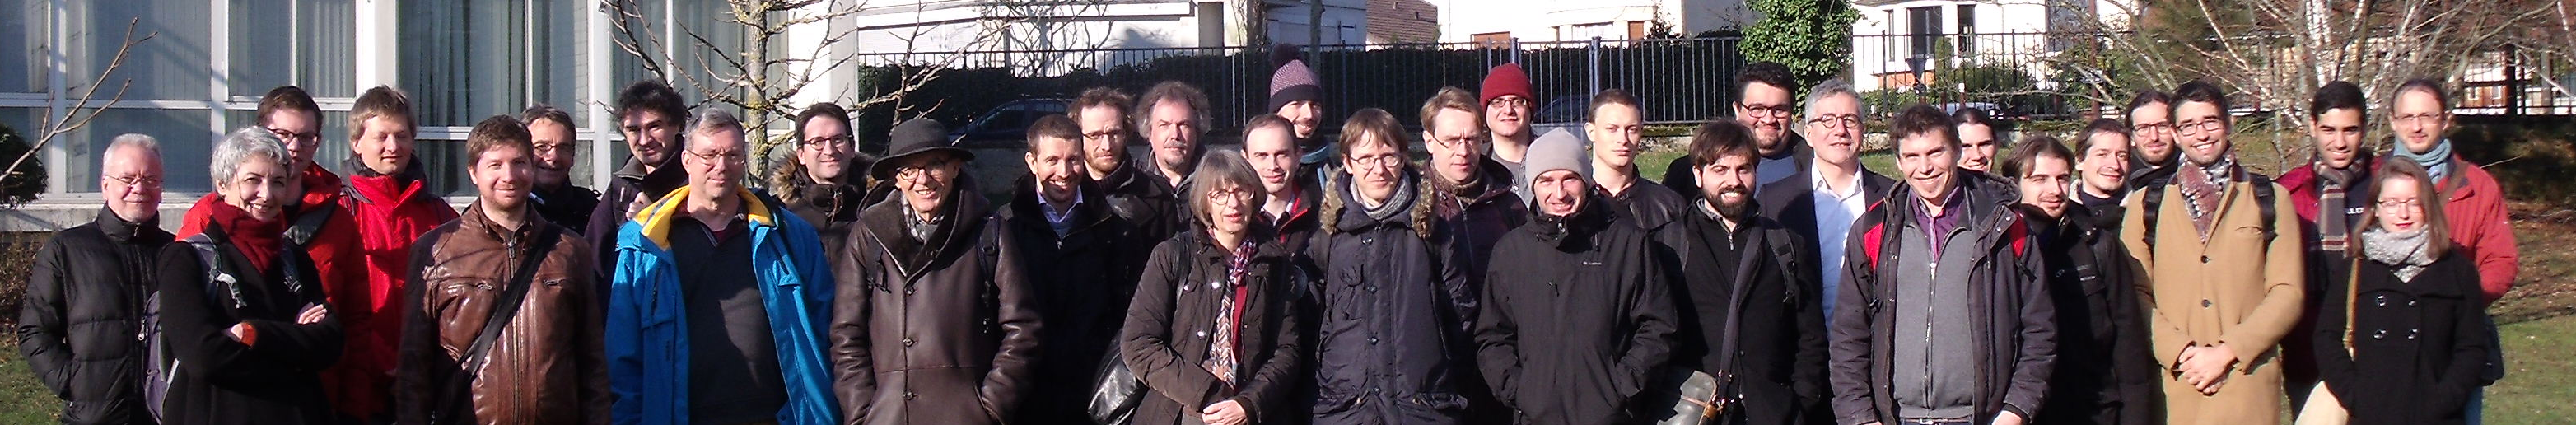
\includegraphics[height=2cm]{photo.png}
\end{center}
During this meeting, the idea of making this proof of concept a
European infrastructure emerged.  Since then, colleagues from Belgium,
Germany, Romania, Serbia, Sweden, and the United Kingdom, from
academia and industry, have manifested interest in participating in
this effort.  These researchers and engineers are ready to contribute
to develop this encyclopedia, aiming at sharing proofs, under a
creative commons licence, making them findable, accessible,
interoperable, and reusable.
\end{framed}

\newpage
~\vfill
\begin{framed}
\vspace*{-0.5cm}
\begin{center}
{\bf \Large How do proofs contribute to safety and security of software?}
\end{center}

Imagine the following casino game. At the beginning, a player is given
eleven euros. At each round, she throws a six-sided die. If the
results is a six, then the game ends.  If it is a five, a four, a
three, or a two, she is given twice the amount of money she already
has. If it is a one she loses two euros, if she has at least two.
When the game ends, the player wins the money she got, except if she
has zero, in which case she loses one million euros.

This game can be modeled by programme $p$
%import random
\begin{verbatim}
n = 11
stay = True;
while stay:
    roll = random.randint(1,6)
    if roll == 6:
        stay = False
    else:
        if roll >= 2:
            n = n + 2 * n
        else:
            if (n >= 2):
                n = n - 2
print(n)
\end{verbatim}

To be on the safe side, the player wants to be sure, before starting
playing, that she will never finish with zero.  And indeed, at all times
the content of the variable {\tt n} is an odd number,
thus it cannot be zero. This property ``nothing bad happens'' is
called the ``safety'' of this program. This property is a
consequence of two simple theorems of arithmetic:
$$\forall x~(\mbox{\it odd}(x) \Rightarrow \mbox{\it odd}(x + 2 * x))$$
$$\forall x~(\mbox{\it odd}(x) \Rightarrow \mbox{\it odd}(x - 2))$$
Hence, verifying the safety of this programme
%, that is that the proposition ${\mbox{\it safe}}(p)$ holds,
amounts to prove these two theorems.

A tiny bug in the program, for instance replacing the {\tt 2} by a
{\tt 3} in the instruction {\tt n = n + 2 * n} makes the programme unsafe
as shown by the sequence $11, 9, 7, 5, 3, 1, 4, 2, 0$. Yet, testing
this program will, most likely, not reveal this bug, since it only manifests
very rarely.  In contrast, attempting to prove the correctness of this
program will
reveal the bug as it is impossible to prove the proposition
$$\forall x~(\mbox{\it odd}(x) \Rightarrow \mbox{\it odd}(x + 3 * x))$$
\end{framed}
\vfill~
\pagebreak
~\vfill
\begin{framed}
\vspace*{-0.5cm}
\begin{center} {\bf \Large Non-trivial mathematics are sometimes
needed to verify that a program is correct}
\end{center}

Prime numbers are used in a wide variety of applications:
pseudo-random number generation, cryptographic algorithms, etc.  Thus,
verifying the correctness of complex primality testing algorithms is
critical.

To do so, we need first to define primality, for instance
\begin{verbatim}
Definition prime p := 1 < p /\ (forall n, 1 < n < p -> ~ (n | p)).
\end{verbatim}

To lower the cost of primality testing, we use tests that are more
efficient than the naive use of the definition.  For instance, a very
simple improvement is to test the divisibility of the considered
number, not by each of the smaller natural numbers, but only up to its
square root.  Indeed, if a natural number $p$ can be factored into the
product of two smaller natural numbers $m$ and $n$, one of them has to
be smaller than or equal to the square root of $p$.  Therefore, one
could give the following more complex, but more efficient, definition.

\begin{verbatim}
Definition prime' p :=
  1 < p /\ (forall n, (1 < n /\ (n * n) <= p) -> ~ (n | p)).
\end{verbatim}

To ensure that these definitions are equivalent one needs to prove
the following statement.

\begin{verbatim}
Theorem prime_alt : forall p, prime' p <-> prime p.
\end{verbatim}

It would have been easy to introduce a small bug
in the new definition.  For example, one could have written
\verb!(n * n) < p!, instead of \verb!(n * n) <= p!.

\begin{verbatim}
Definition prime'' p :=
  1 < p /\ (forall n, (1 < n /\ (n * n) < p) -> ~ (n | p)).
\end{verbatim}
This would have resulted in accepting squares of primes as primes.

Yet, attempting to prove the equivalence of these two definitions would
have revealed the bug, as they cannot be proven to be equivalent.
\end{framed}
\vfill~
\pagebreak
\begin{framed}
  \vspace*{-0.5cm}
  \begin{center}
    {\bf \Large What is a formal proof? What is a proof system?}
    \end{center}

Since Antiquity, we have known that
proofs, both purely mathematical ones, as in Euclid's elements or the
recent proof of the Kepler's conjecture by Thomas Hales, and proofs used
to establish the safety and security of software, can be built with a
limited number of rules, for example
\begin{itemize}
\item From $A \Rightarrow B$ and $A$, deduce $B$.
\item From $A$, deduce $A~\mbox{\it or}~B$.
\item etc.
\end{itemize}
Yet for most of mathematical history, proofs have been written in
a pidgin of natural language and mathematical formulas. When proofs are
very long (as it is often the case for the proofs used in safety and security,
but also for some proofs in pure mathematics), mistakes are
very difficult to detect. For instance, dozens of wrong proofs of
the parallel postulate have been given through history, sometimes by the
best of mathematicians such as Ptolémée, Proclus, al-Haytam, Tacket,
Clairaut, Legendre, etc.

In the 1960s, Robin Milner and Nicolaas De Bruijn noticed that the
correctness of a mathematical proof could be checked by a
computer. This led to the development of the two first proof systems
in history: Milner's LCF and De Bruijn's Automath.  From
the axioms
$$\forall x~(\mbox{\em philosopher}(x) \Rightarrow \mbox{\em human}(x))$$
$$\forall x~(\mbox{\em human}(x) \Rightarrow \mbox{\em mortal}(x))$$
we can deduce
$$\forall x~(\mbox{\em philosopher}(x) \Rightarrow \mbox{\em mortal}(x))$$
In the language implemented in Automath, this proof is written
$$\lambda x \lambda h~(g~x~(f~x~h))$$
\end{framed}

\vfill

\begin{framed}
\vspace*{-0.5cm}
  \begin{center}
{\bf \Large What is a theory?}
\end{center}

Deduction rules such as ``From $A \Rightarrow B$ and $A$, conclude
$B$'' are universal, but building proofs requires more rules, that are
often specific to a domain of knowledge and are called
``axioms''. Examples are the axioms of geometry, the axioms of
arithmetic, etc. These axioms constitute a theory.

At the beginning of the 20$^{\mbox{\footnotesize th}}$ century, an
axiomatic theory, {\em set theory}, has been proposed to express all
mathematical proofs. In the first half of the 20$^{\mbox{\footnotesize
    th}}$ century a few variants of set theory have been proposed, as
well as a few alternatives (such as \emph{Simple type theory}).  But
because these theories had not been designed for being implemented on
a computer, each proof system such as Coq, Isabelle/HOL, Mizar,
Atelier B, etc. implements its own theory.  Thus the rise of
computer-checked formal proofs has led to a multiplication of
alternative theories for mathematics.

This is the major obstacle to interoperability between proof systems.
\end{framed}
\pagebreak

%%% Local Variables:
%%%   mode: latex
%%%   mode: flyspell
%%%   ispell-local-dictionary: "english"
%%% End:
